\documentclass[11pt,a4paper]{article}
\usepackage[margin=1in]{geometry}
\usepackage[T1]{fontenc}
\usepackage[utf8]{inputenc}
\usepackage{lmodern}
\usepackage{hyperref}
\usepackage{enumitem}
\usepackage{xurl}
\usepackage{tikz}
\usepackage{float}
\usetikzlibrary{arrows.meta, positioning, shapes.geometric}
\hypersetup{colorlinks=true,linkcolor=blue,urlcolor=blue}
\newcommand{\codepath}[1]{\path{#1}}
\tikzset{box/.style={rectangle,draw,rounded corners,align=center,inner sep=3pt,minimum width=36mm},decision/.style={diamond,draw,aspect=2.1,align=center,inner sep=2pt},line/.style={-Latex}}

\title{Phase-2 gem5: Deliverable 9 (CI Integration)}
\author{Senior Systems Architecture}
\date{\today}

\begin{document}
\maketitle

\section{Technical Description}
CI integration for gem5 enforces deterministic regression gates before merge.

\section{Implementation Fulfillment}
Reusable checks exist (\codepath{Phase-2/tests/check_adapter_fixtures.py}, \codepath{Phase-2/tests/check_determinism.py}, \codepath{Phase-2/run_cross_target_suite.py}).\\
Current implementation gap: no dedicated \codepath{.github/workflows/phase2-ci.yml}.

\section{Design \& Architecture}
CI should run fast target checks in PR lane and heavier replay/nightly checks separately. Failure artifacts must be retained for triage.

\subsection*{Function Flowchart}
\begin{figure}[H]
\centering
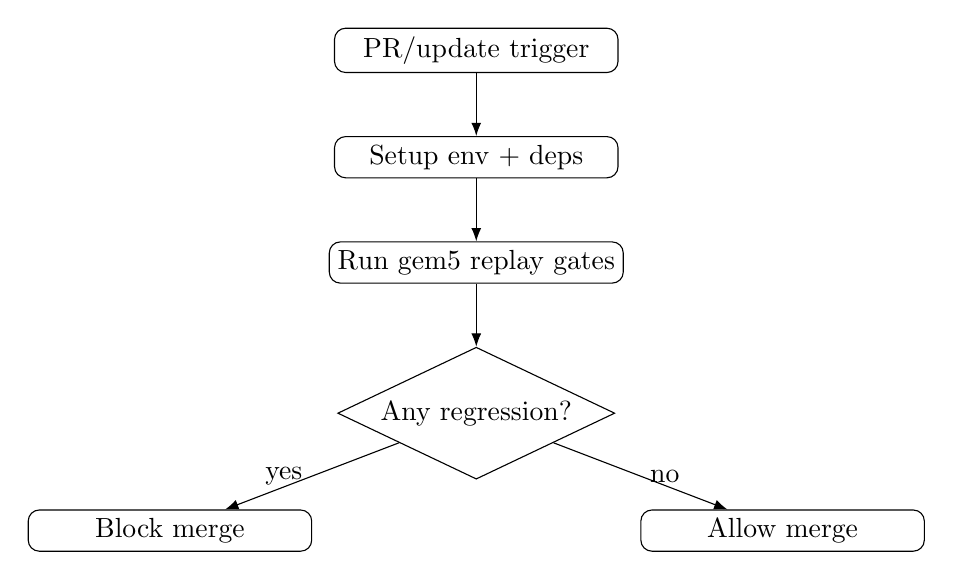
\begin{tikzpicture}[node distance=8mm and 12mm]
\node[box] (a) {PR/update trigger};
\node[box, below=of a] (b) {Setup env + deps};
\node[box, below=of b] (c) {Run gem5 replay gates};
\node[decision, below=of c] (d) {Any regression?};
\node[box, below left=of d] (e1) {Block merge};
\node[box, below right=of d] (e2) {Allow merge};
\draw[line] (a) -- (b);
\draw[line] (b) -- (c);
\draw[line] (c) -- (d);
\draw[line] (d) -- node[left]{yes} (e1);
\draw[line] (d) -- node[right]{no} (e2);
\end{tikzpicture}
\caption{gem5 CI Integration Flow}
\end{figure}

\end{document}
